\documentclass[border=10pt]{standalone}

\usepackage{tikz}
\usepackage{tikzsymbols}
\usetikzlibrary{calc,patterns,shapes.geometric}

\def\centerarc[#1](#2)(#3:#4:#5){\draw[#1] ($(#2)+({#5*cos(#3)},{#5*sin(#3)})$) arc (#3:#4:#5);}

\begin{document}
	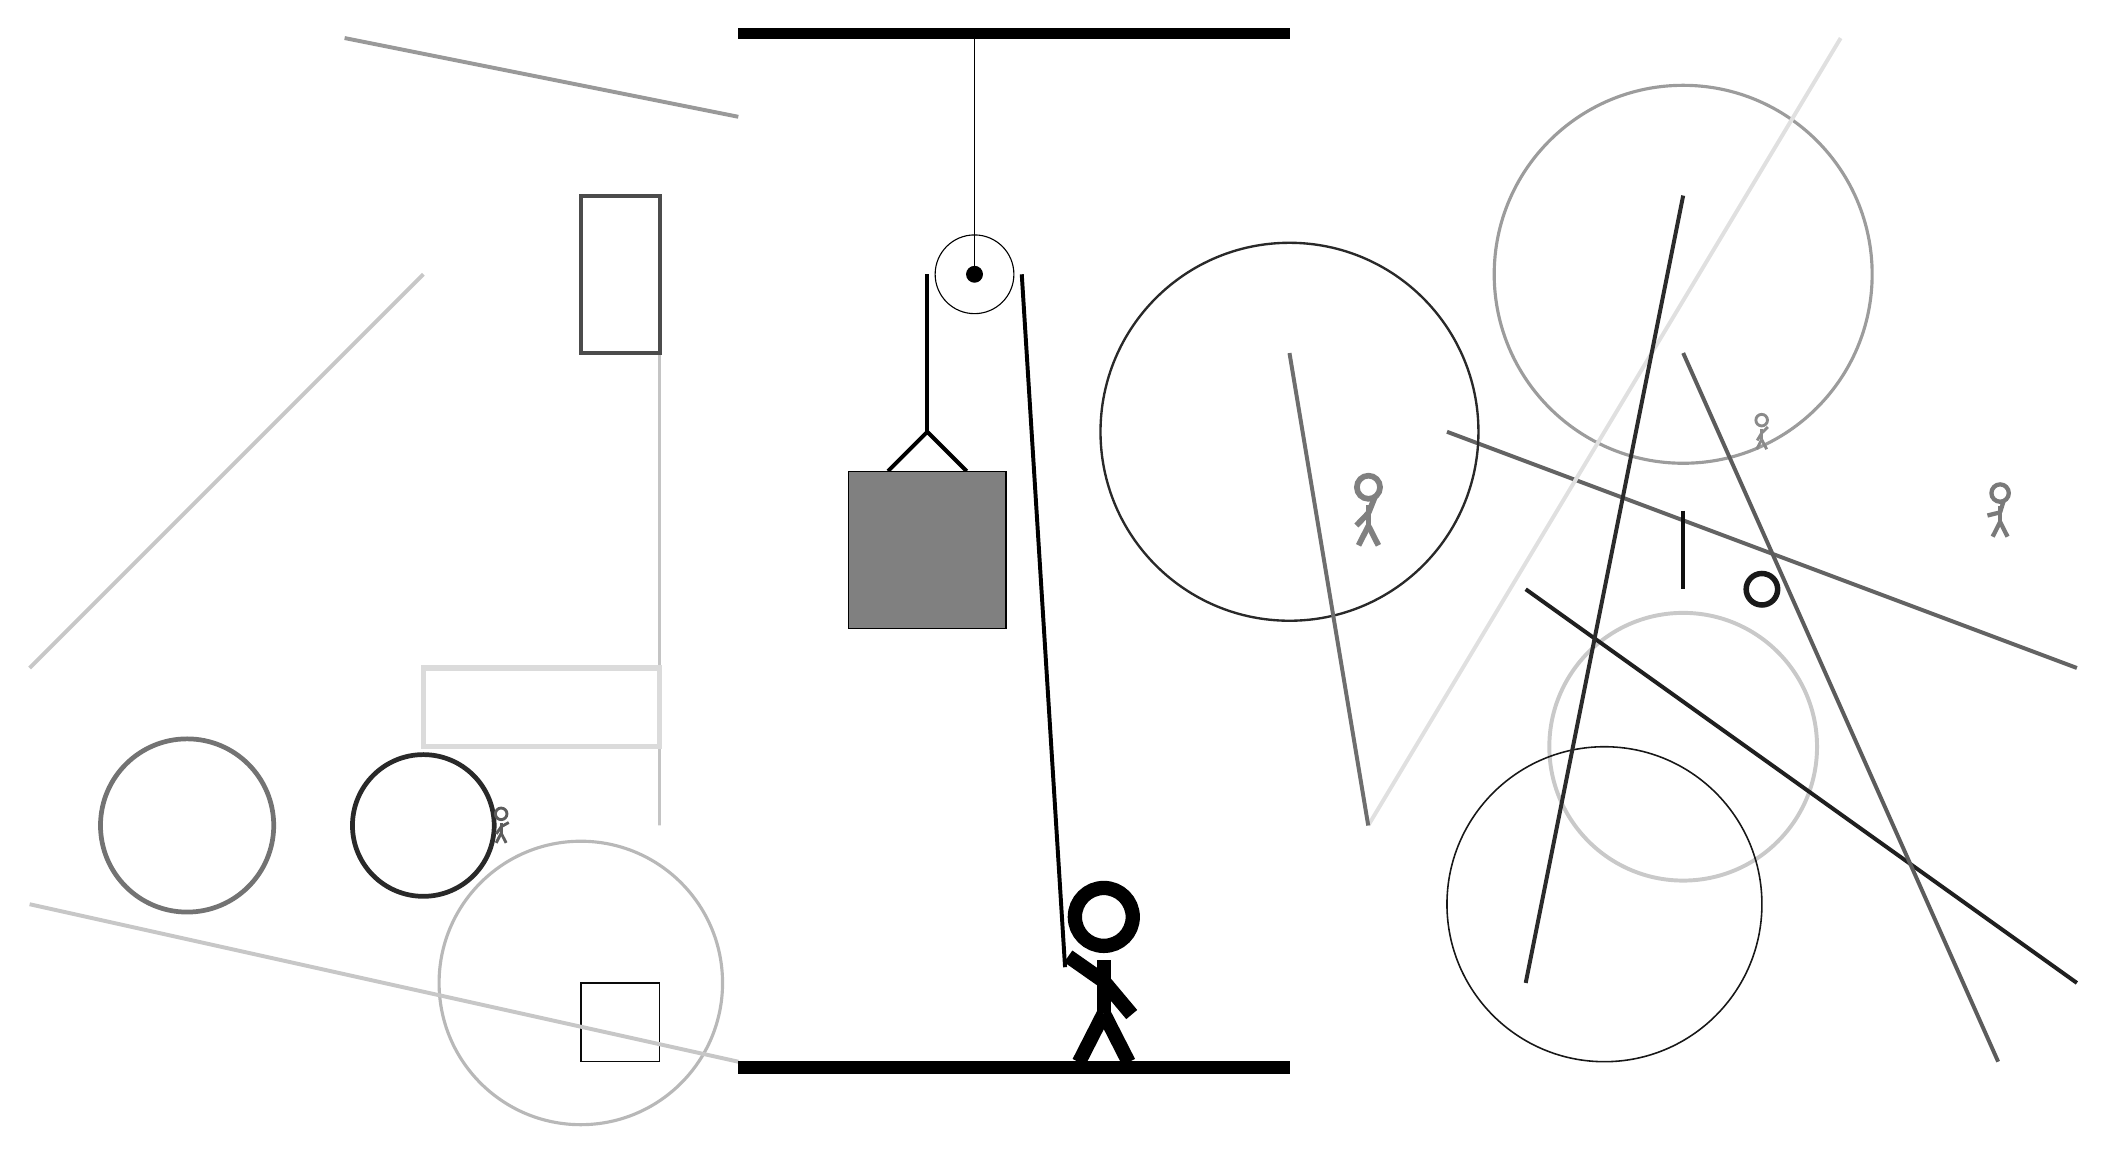
\begin{tikzpicture}
		%%%%% START %%%%%
		
		\draw[fill=black] (-2, 10) rectangle (5, 10.125);
		
		\draw (1, 7) circle (0.5);
		\draw[fill=black] (1, 7) circle (0.1);
		\draw (1, 10) -- (1, 7);
		
		\draw[line width=0.5mm] (-0.1, 4.5) -- (0.4, 5.0) -- (0.9, 4.5);
		\draw[fill=black!50] (-0.6, 4.5) rectangle (1.4, 2.5);
		
		\draw [line width=0.4mm, color=black!39](10, 7) circle (2.4);
		
		\draw [line width=0.6mm, color=black!84](-6, 0) circle (0.9);
		\draw [line width=0.5mm, color=black!21](10, 1) circle (1.7);
		\node[line width=0.2mm, color=black!50] at (6, 4) {\Strichmaxerl[4][46][68]};
		\draw[line width=0.5mm, color=black!61](7, 5) -- (15, 2);
		\draw[line width=0.5mm, color=black!22](-6, 7) -- (-11, 2);
		
		\draw[line width=0.5mm, color=black!94](10, 4) -- (10, 3);
		\draw [line width=0.4mm, color=black!28](-4, -2) circle (1.8);
		\draw[line width=0.5mm, color=black!88](8, 3) -- (15, -2);
		\node[line width=0.3mm, color=black!46] at (11, 5) {\Strichmaxerl[2][59][44]};
		\node[line width=0.7mm, color=black!52] at (14, 4) {\Strichmaxerl[3][14][73]};
		\draw[line width=0.3mm, color=black!23] (-3, 6) rectangle (-3, 0);
		\draw [line width=0.3mm, color=black!84](5, 5) circle (2.4);
		\draw [line width=0.2mm, color=black!91](9, -1) circle (2.0);
		\draw [line width=0.6mm, color=black!55](-9, 0) circle (1.1);
		\draw[line width=0.5mm, color=black!70] (-3, 8) rectangle (-4, 6);
		
		\draw[line width=0.2mm, color=black!96] (-4, -3) rectangle (-3, -2);
		\draw[line width=0.5mm, color=black!22](-2, -3) -- (-11, -1);
		\draw[line width=0.5mm, color=black!12](6, 0) -- (12, 10);
		\node[line width=0.5mm, color=black!64] at (-5, 0) {\Strichmaxerl[2][56][29]};
		\draw [line width=0.7mm, color=black!90](11, 3) circle (0.2);
		
		\draw[line width=0.5mm, color=black!57](5, 6) -- (6, 0);
		\draw[line width=0.5mm, color=black!83](8, -2) -- (10, 8);
		\draw[line width=0.5mm, color=black!40](-7, 10) -- (-2, 9);
		\draw[line width=0.5mm, color=black!64](10, 6) -- (14, -3);
		
		\draw[line width=0.7mm, color=black!14] (-3, 2) rectangle (-6, 1);
		
		\draw[line width=0.5mm] (0.4, 7) -- (0.4, 5.0);
		\centerarc[line width=0.5mm](1, 7)(0:180:0.6);
		\draw[line width=0.5mm](1.6, 7) -- (2.15, -1.8);
		
		\node at (2.6, -1.9) {\Strichmaxerl[10][-35][-50]};
		
		\draw[fill=black] (-2, -3) rectangle (5, -3.15);
		
		%%%%% END %%%%%
	\end{tikzpicture}
\end{document}